\section{System's Perspective}
% Double check that for all the weekly tasks (those listed in the schedule) you include the corresponding information.

\subsection{Design and Architecture}
% Design and Architecture of Our ITU-MiniTwit Systems
% sabrina - see report branch
Our version of MiniTwit uses Docker Swarm with 6 virtual machines (vms) and a separate vm for the database. The API and back-end are both built in Golang. The web framework is built using Gin. PostgreSQL is used for our database. Prometheus is used in conjunction with Grafana for monitoring, and Loki is used for logging.  

\subsection{Dependencies of Our ITU-MiniTwit System}
%  On All Levels of Abstraction and Development Stages
% That is, list and briefly describe all technologies and tools you applied and depend on.
% Jakob
The following list includes all technologies and tools used in our system.

\textbf{Web Application:}
\begin{itemize}
    \item \textbf{Go} - Chosen programming language for our back-end.
    \begin{itemize}
        \item \textbf{Gin} - Web framework for Go, helps with creating endpoints.
        \item \textbf{GORM} - used as an ORM library for Golang
        \item \textbf{bcrypt} - package used for hashing the stored passwords.
        \item \textbf{Prometheus client} - used for creating metrics that are tracked and displayed on the endpoint ``metrics"
        \item \textbf{GoDotEnv} - used for storing ``secret" variables.
    \end{itemize}
    \item \textbf{HTML} - Markup language used for displaying data on the front-end, following the Go Template Syntax.
    \item \textbf{CSS} - Styling language to make our displayed data look nice.
    \item \textbf{PostgreSQL} - Query language to store our data in a database
\end{itemize}
\textbf{Monitoring Setup:}
\begin{itemize}
    \item \textbf{Prometheus} - Used to create monitor metrics of our systems. These include the number requests to our endpoints and the status of our system (i.e. is our system up).
    \item \textbf{Loki} - The ``Loki driver" plugin is used as our logger. It collects all logs from our Docker containers and aggregates them.
    %Same principle as Prometheus, but for logs %connected to docker via the 'loki driver' docker plugin
    \item \textbf{Grafana} - Used to display our dashboards. Prometheus and Loki are added as data sources here, and we have dashboards configured to display both the Loki logs and the Prometheus metrics.
\end{itemize}
\textbf{Infrastructure:}
\begin{itemize}
    \item \textbf{Docker} - Builds our application 
    \item \textbf{Docker swarm} - management and scaling of Docker containers
    \item \textbf{Linux} (Ubuntu?)
    \item \textbf{Digital Ocean} - Our choice  of cloud service provider
\end{itemize}
\textbf{CI/CD:}
\begin{itemize}
    \item \textbf{Vagrant. Working on converting to Terraform} - Script for our Continuous Deployment to Digital Ocean
    \item \textbf{GitHub actions} - Pipeline for Continuous Integration
    \begin{itemize}
        \item \textbf{Cypress} - UI/end-to-end tests, automatically run in the pipeline % (We need to consider what kind of tests we have, what kinds are missing, among the following: UI, end-to-end, integration)
        \item GitHub actions for docker
        \item \textbf{appleboy/ssh-action@v0.1.8} - executing remote ssh commands.
    \end{itemize}
    \item \textbf{SonarCloud} - Checking code quality 
    \item \textbf{CodeClimate} - Also checking code quality % (added later)
    \item \textbf{ShellCheck and govulncheck} - analyses code/commands checks for faults % (added later)
\end{itemize}
\textbf{Development:}
\begin{itemize}
    \item \textbf{GitHub} - Storing the project, uses Git as version control
    \item \textbf{Python} - For simulator tests
    \item \textbf{Docker compose} - Building the application with one command
    \item \textbf{OWASP ZAP} - Pen-testing our website
\end{itemize}
\textbf{Documentation:}
\begin{itemize}
    \item \textbf{LaTeX} - Writing this report
    \item \textbf{Markdown} - Lightweight way of writing documents, used e.g. in our README and SLA
    \item \textbf{ChatGPT} - Chatbot, helps us getting quick answers % (writing the SLA)
\end{itemize}

\subsection{Important Interactions of Subsystems}
% dee
As shown in Fig. \ref{fig:subsystems} the MiniTwit app is dependent on the database and Grafana, which are both separate containers. Images for both Prometheus and Grafana are configured in the \textit{docker-compose.yml}. Both have a specified port and volumes pointing to corresponding configuration files. Within the Prometheus configuration we have set up to scrape data from MiniTwit.

Grafana has a volume built on the contents of the directory \textbf{provisioning} in our repository. Within this is a yaml containing a list of data sources for Grafana. Here both Prometheus and Loki are added as data sources.

Loki receives the logs from all the other containers.

\begin{figure}[H]%[!ht]
\begin {center}
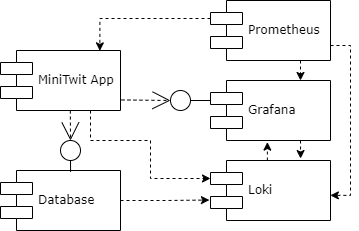
\includegraphics[width=0.5\textwidth]{figures/subsystems.drawio.png}
\caption{Subsystem interaction}
\label{fig:subsystems}
\end {center}
\end{figure}

\subsection{The Current State of Our Systems}

From a purely transcendental point of view, the quality of the code is subpar. 

It is especially the \emph{reliability} of the system which is questionable, with a large amount of downtime caused by an unknown error (this is expanded on in \ref{monitoring}). Static code analysis, shown in Fig. \ref{fig:sonarcloud} does not, however, not detect many large reliability issues.

\begin{figure}[h]
\centering
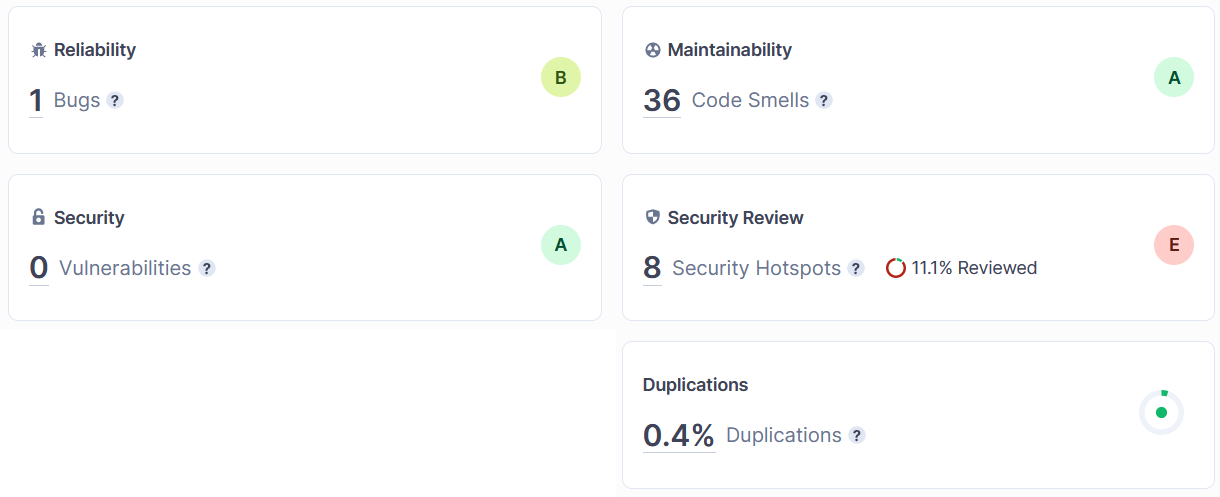
\includegraphics[width=0.8\textwidth]{figures/SonarCloudUpdated.png}
\caption{SonarCloud scan results of the development branch.}
\label{fig:sonarcloud}
\end{figure}

\ref{fig:sonarcloud} indicates that the code is \emph{maintainable}. The low complexity of the system also reduces the threshold of when the system is unmaintainable.

The system is \emph{portable} to a certain extent. It is dockerized, and can be deployed on a docker swarm on any machine(s) with docker. The current terraform deploy script does however rely on specifically using digital ocean as IaaS provider.

\subsection{Chosen Licence Compatibility with Direct Dependencies}
% Finally, describe briefly, if the license that you have chosen for your project is actually compatible with the licenses of all your direct dependencies.
% dont need to check prometheus, grafana, loki
% check code dependencies: gorm, gin, etc
% sabrina

We chose the MIT License for our project and to ensure compatibility with our direct code dependencies we checked the licenses for each package we used (Table \ref{table:dep}).

\begin{table}[!h]
\centering
\begin{tabular}{lll}
\toprule
Language & Package & License \\ 
\midrule
Go & \href{https://github.com/gin-gonic/gin}{Gin} & \href{https://github.com/gin-gonic/gin/blob/master/LICENSE}{MIT} \\ 
Go & \href{https://github.com/go-gorm/gorm}{GORM} & \href{https://github.com/go-gorm/gorm/blob/master/License}{MIT} \\ 
Go & \href{https://pkg.go.dev/golang.org/x/crypto/bcrypt}{crypto (bcrypt)} & \href{https://pkg.go.dev/golang.org/x/crypto/bcrypt?tab=licenses}{BSD 3-Clause} \\ 
Go & \href{https://github.com/prometheus/client_golang}{Prometheus client} & \href{https://github.com/prometheus/client_golang/blob/main/LICENSE}{Apache License 2.0} \\ 
Go & \href{https://github.com/joho/godotenv}{GoDotEnv} & \href{https://github.com/joho/godotenv/blob/main/LICENCE}{MIT} \\ 
Go & \href{https://github.com/stretchr/testify}{testify} & \href{https://github.com/stretchr/testify/blob/master/LICENSE}{MIT} \\ 
Python & \href{https://github.com/psf/requests}{requests} & \href{https://github.com/psf/requests/blob/main/LICENSE}{Apache License 2.0} \\ 
\bottomrule
\end{tabular}
\caption{Code dependencies and their licenses}
\label{table:dep}
\end{table}

The MIT, BSD 3-Clause, and Apache License are compatible with each other as they are permissive and unlike copyleft licenses such as the GNU General Public License (GPL), do not require modifications and derivative works to be distributed under the same copyleft license.

Permissive licenses have minimal requirements for usage and redistribution and typically only ask for the inclusion of the original copyright notice and a copy of the license text when distributing the software. They  are designed to be accommodating, allowing developers to use the code in various projects, including proprietary ones.



% Description of 'current state of system' (use static code analysis e.g.)

% Choice of license (is it compatible with direct dependencies)
